\section{Przykłady działania aplikacji}
Po uruchomieniu aplikacji widzimy 3 okna:

Po lewej znajduje się główne okno GUI, po prawej u góry jest okno terminala z którego uruchomiono GUI, natomiast niżej znajduje się okno na którym uruchomiony jest serwer.
Jak widać na obrazie poniżej, aplikacja serwerowa wypisuje na standardowe wyjście informacje takie jak zawartość zapytania odebrana od GUI, oraz czas jaki zajęło serwerowi wygenerowanie obrazu.
\begin{figure}[H]
    \centering
    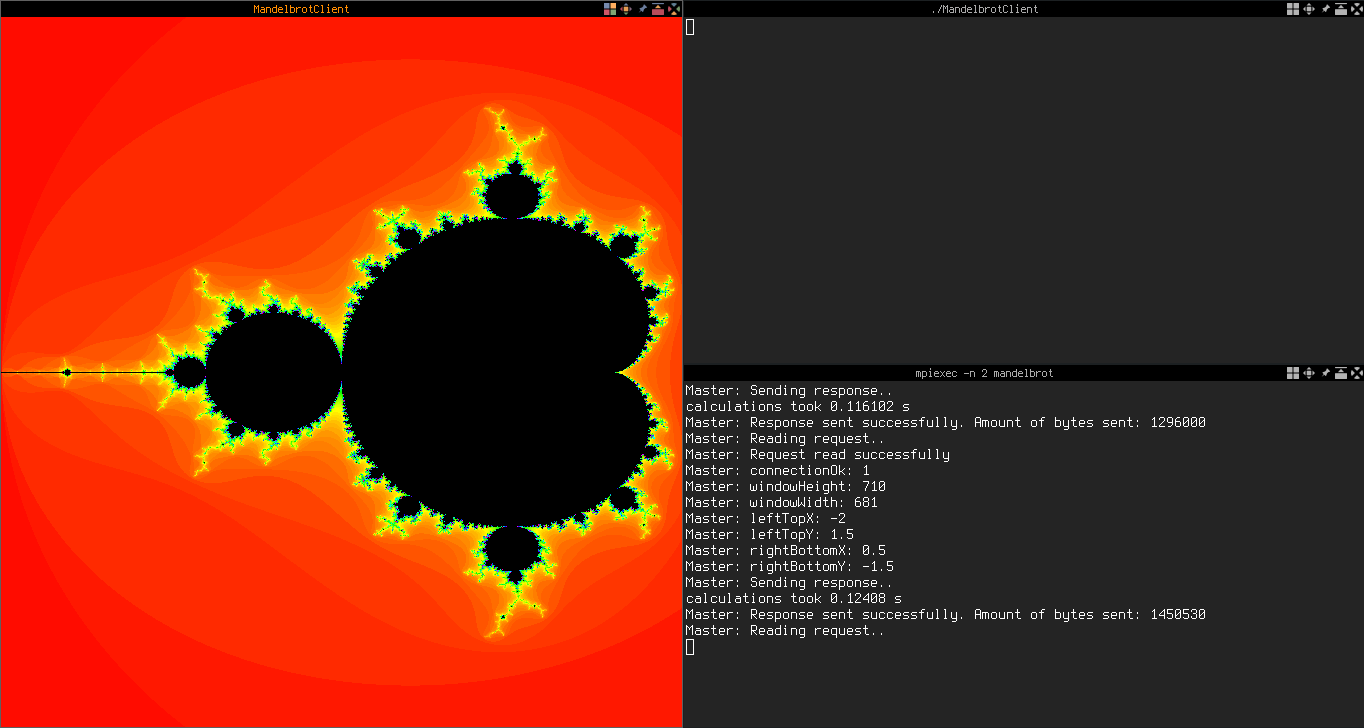
\includegraphics[width = \textwidth]{img/ex1.png}
\end{figure}

Aplikacja odpowiedzialna za interfejs użytkownika również wypisuje dane diagnostyczne na standardowe wyjście.
\begin{figure}[H]
    \centering
    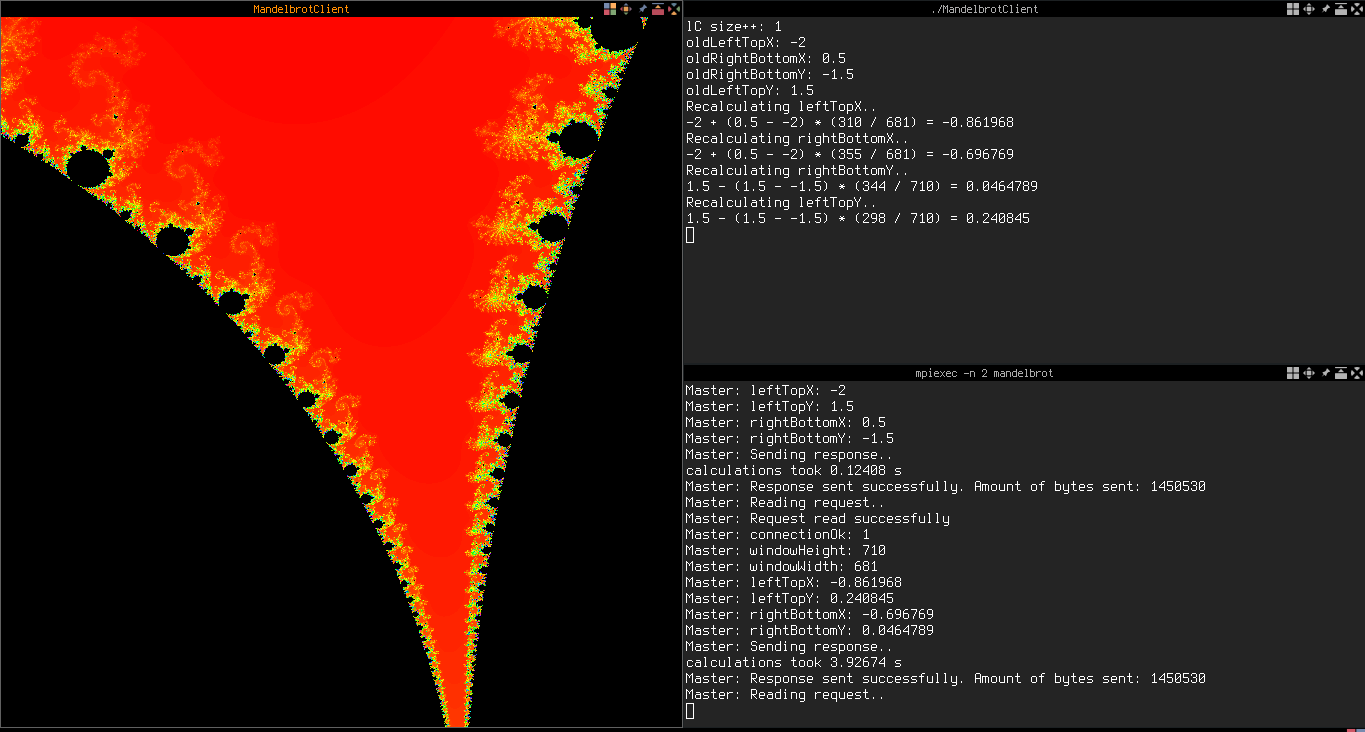
\includegraphics[width = \textwidth]{img/ex2.png}
\end{figure}

Jak można zaobserwować na poniższym obrazie aplikacja pozwala uzyskać znaczne przybliżenie na elementy zbioru.
\begin{figure}[H]
    \centering
    
\includegraphics[width = 0.7\textwidth]{img/ex3.png}
\end{figure}